\documentclass[varlength,tikz]{standalone}

\usetikzlibrary{arrows,shapes,snakes,automata,calc,matrix,backgrounds,petri, positioning}

\begin{document}
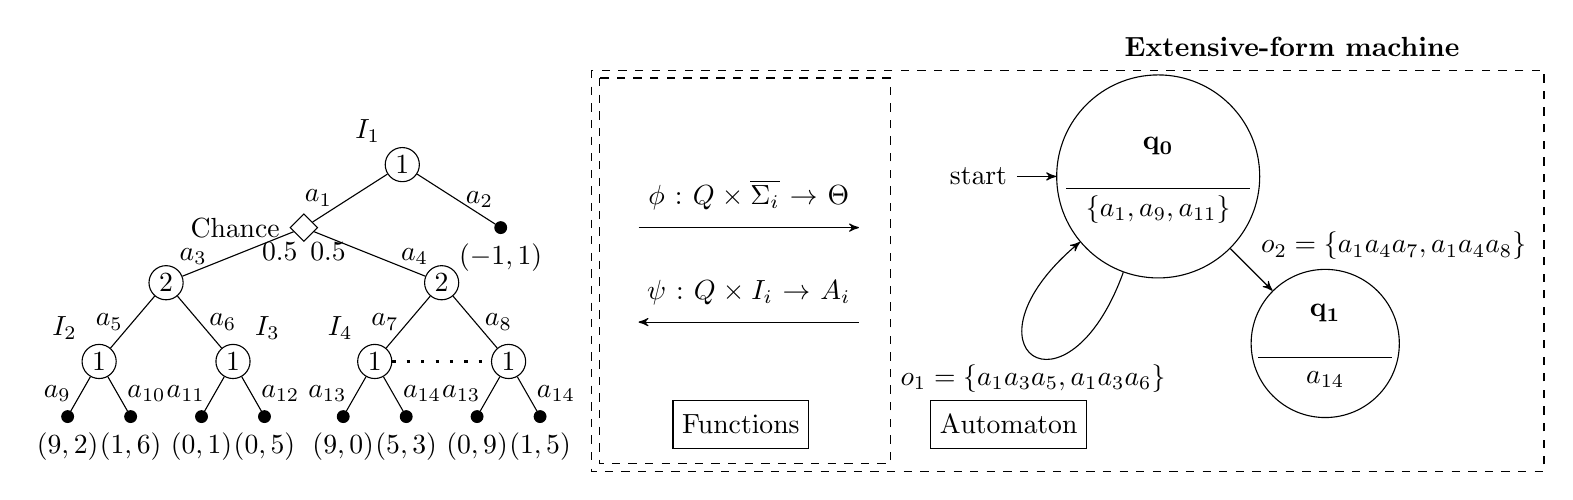
\begin{tikzpicture}[node distance=1.3cm,>=stealth',bend angle=45,auto]
  \begin{scope}
  \tikzstyle{solid node}=[circle,draw,inner sep=1.5,fill=black]
  \tikzstyle{hollow node}=[diamond,draw,inner sep=2.5]
    \tikzstyle{p1 node}=[font={$1$},circle,draw,inner sep=1.5]
  \tikzstyle{p2 node}=[font={$2$},circle,draw,inner sep=1.5]
  \tikzstyle{level 1}=[level distance=8mm,sibling distance=2.5cm]
  \tikzstyle{level 2}=[level distance=7mm,sibling distance=3.5cm]
  \tikzstyle{level 3}=[level distance=10mm,sibling distance=1.7cm]
  \tikzstyle{level 4}=[level distance=7mm,sibling distance=0.8cm]
  \node(0)[p1 node, label=above left:$I_1$]{}
      child{node[hollow node,label=left:Chance]{}{
      child{node[p2 node]{}{
%      	child{node[p1 node]{}{ 
%		child{node[solid node,label=below:{$(1,1)$}]{} edge from parent node[left]{$a_8$}}
%      	 	child{node[solid node,label=below:{$(2,4)$}]{} edge from parent node[right]{$a_9$}}
%      		edge from parent node[left]{$a_3$}}}
      	child{node[p1 node, label=above left:$I_2$]{}{
      		child{node[solid node,label=below:{$(9,2)$}]{} edge from parent node[left]{$a_{9}$}}
      	 	child{node[solid node,label=below:{$(1,6)$}]{} edge from parent node[right]{$a_{10}$}}
      	  	edge from parent node[left]{$a_5$}}}
	child{node[p1 node, label=above right:$I_3$]{}{
      		child{node[solid node,label=below:{$(0,1)$}]{} edge from parent node[left]{$a_{11}$}}
      	 	child{node[solid node,label=below:{$(0,5)$}]{} edge from parent node[right]{$a_{12}$}}
      	  	edge from parent node[right]{$a_6$}}}
       	edge from parent node[left,xshift=25]{$a_3\quad\quad0.5$}}
       	}
      child{node[p2 node]{}{
%      		child[level distance=7mm,sibling distance=8mm]{node[solid node,label=below:{$(2,1)$}]{} edge from parent node[left]{$a_6$}}
%      	 	child[level distance=7mm,sibling distance=8mm]{node[solid node,label=below:{$(2,5)$}]{} edge from parent node[right]{$a_7$}}
      	 child{node[p1 node, label=above left:$I_4$]{}{
      		child{node[solid node,label=below:{$(9,0)$}]{} edge from parent node[left]{$a_{13}$}}
      	 	child{node[solid node,label=below:{$(5,3)$}]{} edge from parent node[right]{$a_{14}$}}
      	  	edge from parent node[left]{$a_7$}}}
	child{node[p1 node]{}{
      		child{node[solid node,label=below:{$(0,9)$}]{} edge from parent node[left]{$a_{13}$}}
      	 	child{node[solid node,label=below:{$(1,5)$}]{} edge from parent node[right]{$a_{14}$}}
      	  	edge from parent node[right]{$a_8$}}}
      	edge from parent node[right,xshift=-25]{$0.5\quad\quad a_4$}}
      	}
      	edge from parent node[left,xshift=-3]{$a_1$}}
      	}
      	child{node[solid node,label=below:{$(-1,1)$}]{} edge from parent node[right]{$a_{2}$}}
    ;
    \draw[loosely dotted,very thick](0-1-2-1)to(0-1-2-2);
  \end{scope}

  \begin{scope}[xshift=9.6cm,yshift=-0.15cm,initial distance=0.5cm,node distance=3cm]
    % Second net
    \node[initial,state, inner sep=0cm] (A)                    {\begin{tabular}{c} $\mathbf{q_0}$ \\ ~ \\$\{a_1, a_9, a_{11}\}$ \end{tabular}};
  \node[state]         (B) [below right of=A] {\begin{tabular}{c} $\mathbf{q_1}$ \\ ~ \\ $a_{14}$ \end{tabular}};

  \path[->] (A) edge              node {$o_2=\{a_1a_4a_7, a_1a_4a_8\}$} (B)
  		      edge [out=250,in=220,looseness=8] node[below] {$o_1=\{a_1a_3a_5,a_1a_3a_6\}$}(A);
  \end{scope}
  \draw[-] (8.43,-0.3) -- (10.77,-0.3);
  \draw[-] (10.87,-2.45) -- (12.57,-2.45);
\draw[->] (3.0,-0.8) -- (5.8,-0.8)
	node [above=1mm,midway,text width=3cm,text centered]
      {$\phi:Q\times {\overline{\Sigma_i}}\rightarrow \Theta$};
\draw[<-] (3.0,-2.0) -- (5.8,-2.0)
	node [above=1mm,midway,text width=3cm,text centered]
      {$\psi:Q\times I_i\rightarrow A_i$};
      \draw[dashed] (2.4,1.2) rectangle (14.5,-3.9);
       \draw[dashed] (2.5,1.1) rectangle (6.2,-3.8);
       \node at (11.3,1.5) {\bf Extensive-form machine};
       \node[draw, minimum height=0.6cm] at (4.3,-3.3) {Functions};
       \node[draw, minimum height=0.6cm] at (7.7,-3.3) {Automaton};
\end{tikzpicture}
\end{document}